\documentclass[journal]{IEEEtran}
\usepackage{graphicx} % Required for inserting images
\usepackage{caption} % For captions
\usepackage[utf8]{inputenc}

% *** CITATION PACKAGES ***
\usepackage{cite}
% cite.sty was written by Donald Arseneau
% V1.6 and later of IEEEtran pre-defines the format of the cite.sty package
% \cite{} output to follow that of the IEEE. Loading the cite package will
% result in citation numbers being automatically sorted and properly
% "compressed/ranged". e.g., [1], [9], [2], [7], [5], [6] without using
% cite.sty will become [1], [2], [5]--[7], [9] using cite.sty. cite.sty's
% \cite will automatically add leading space, if needed. Use cite.sty's
% noadjust option (cite.sty V3.8 and later) if you want to turn this off
% such as if a citation ever needs to be enclosed in parenthesis.
% cite.sty is already installed on most LaTeX systems. Be sure and use
% version 5.0 (2009-03-20) and later if using hyperref.sty.
% The latest version can be obtained at:
% http://www.ctan.org/pkg/cite
% The documentation is contained in the cite.sty file itself.

\graphicspath{ {./images/} }

\title{Comparative Analysis of a Wave Energy Converter Containing a Winch-Based Mechanical Motion Rectifier With Similar Designs}
\author{Philip Paterson}
\date{June 2023}

\begin{document}

\maketitle

\begin{abstract}
    The field of Wave Energy Converters (WECs) is exciting yet underdeveloped. A recent WEC design developed by Joseph Saltsman, named the "Wave Piston," aims to produce energy from waves efficiently and at a lower cost. It sports novel power take-off and extraction subsystems that seem promising. However, due to the Wave Piston being in the early stages of development, a literature review has been conducted in this report to illustrate the Wave Piston's potential compared to other designs.
\end{abstract}

\section{Introduction}
In the transition to clean energy, the ocean is a vast untapped resource that can supply much of the world's energy if utilized correctly. Devices that harness the energy from waves are called Wave Energy Converters (WECs). While there have been efforts to develop WECs, the technology overall is immature and needs more advancements to become viable. We propose that the Wave Piston, a unique WEC design, has the potential to bring us one step closer to a future powered solely by renewables.

\section{Comparing WEC Categories}
With the wide variety of Wave Energy Converter systems out there, many different types of subsystems are associated with these devices. This section will focus on outlining the categories used to classify WECs.

\subsection{Location}
    One main way WEC devices can be classified is based on their location. WECs can be either shoreline, nearshore, or offshore devices \cite{doi:10.1243/09576509JPE782}.
    
    Shoreline devices reside on the shore. While shoreline devices are easier to maintain and are less likely to be damaged by extreme conditions experienced farther into the waters, they also have drawbacks. These include lower wave power due to more shallow water and restrictions related to their disruption of the scenery and needing to design around its local geography \cite{doi:10.1243/09576509JPE782}.
    
    Nearshore WECs can be roughly referred to as devices in "shallow" water, or in water of around less than a quarter of a wavelength deep. Nearshore devices still experience power loss due to shallower waters but can be attached to the seabed, which provides a solid foundation for some WECs \cite{doi:10.1243/09576509JPE782}.
    
    What exactly delineates an offshore WECs is not agreed upon, but for our purposes we will follow the convention that is in waters of greater than 40 meters in depth \cite{boyle2004renewable}. These WECs can harness more energy due to the deeper waters but are harder to construct and maintain and must be able to survive extreme conditions, adding to costs\cite{boyle2004renewable, doi:10.1243/09576509JPE782}.

\subsection{Extraction Technology}
    WECs can be further classified based on their extraction technology, which can be grouped under these three broad categories: oscillating water columns, oscillating body systems, and overtopping systems\cite{en12224329}.

    It has been found that among the three technologies, oscillating body systems have the highest ratio of hydrodynamic efficiency to the characteristic width of the WEC\cite{en12224329}. Heaving systems, better known as point-absorbers, are classified as oscillating body systems. Point absorbers are generally smaller than other WEC devices, mechanically simpler, and can generate power from any wave direction\cite{su14169936, HONG2014329}. These benefits demonstrate the advantage of the Wave Piston being a point absorber. 

\subsection{Power Take-Off System}
    The Power Take-Off (PTO) system of a WEC is the subsystem that converts mechanical energy from the waves into another useful form of energy, like electricity \cite{osti_1897711}.

    Many PTO systems exist, most of which fall under being hydraulic, water, air turbines, mechanical drive, direct-drive electrical generators, electroactive polymers, and triboelectric nanogenerators\cite{osti_1897711}.
    
    Direct-drive electrical generators can either be rotary or linear generators. While rotary generators are highly efficient, they are costly due to the rare earth metals in their permanent magnets\cite{osti_1897711}. Developers are also looking at linear direct-drive generators, which are a promising technology. However, these linear generators are still immature and come with high costs, a small power-to-weight ratio, and a complicated power transmission system\cite{su14169936, Leijon_2008, osti_1897711}.

    Similarly, while electroactive polymers and triboelectric nanogenerators are exciting technologies with a good outlook, they are also immature, and more work needs to be done to develop them\cite{osti_1897711}.

    For the rest of the PTO technologies, Figure 1 summarizes their efficiencies and shows that the mechanical drive has the second-highest efficiency of the PTO technologies\cite{en12224329}.
    \begin{figure}[htbp]
    \centerline{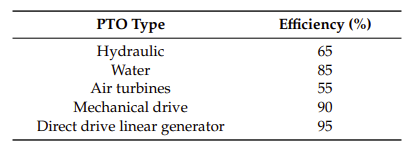
\includegraphics{images/pto_efficiencies_table.png}}
    \caption{Typical PTO Efficiencies. PTO: power take-off}
    \label{fig}
    \end{figure}

\section{Comparing the Wave Piston to similar WECs}
The Wave Piston can be classified as a nearshore point-absorbing WEC with a mechanical drive PTO that consists of two winches that each drive a one-way clutch, respectively, enabling bidirectional energy absorption.

As shown in Section II, the Wave Piston's potential is already high due to its subsystems and characteristics being theoretically more efficient and cost-effective, like the fact that oscillating body WECs have the highest hydrodynamic efficiency relative to their characteristic width or that mechanical drive PTOs have the second highest theoretical efficiency\cite{en12224329}.

While there is no exact match to the Wave Piston design to compare to, there are similar designs, like one that similarly use a winch attached to a counter-weight run along one-way clutches to harness bidirectional motion\cite{LOK20141}. The Wave Piston's mechanical motion rectifier (MMR) avoids some of the pitfalls with counter-weight PTOs, such as the added weight and potential damage from a free-swinging counter-weight\cite{nachev2017comparative}.

Another comparative design is a WEC whose PTO includes a rack-and-pinion system with two-one-way bearings integrated into it to form its MMR\cite{LIANG2017190}. One can speculate that using cables instead of a rack-and-pinion system would be less subject to mechanical stresses, but more work needs to be done to make any conclusion.

Furthermore, from reviewing similar designs, potential problems may occur. Besides the disadvantages listed due to the Wave Piston's category, these issues may include damage from motion that exceeds the Wave Piston's maximum allowed translation, low durability and high maintenance costs due to the bidirectional gears, and the comparatively larger support structure needed for the cables. However, as stated before, no solid claim can be made about the Wave Piston design until it is properly modeled and simulated.

\section{Conclusion}
This report includes a literature review of wave energy converters, their respective subsystems, and how they compare with the Wave Piston design. Just by reviewing the academic work surrounding WECs and similar WEC designs, the Wave Piston design seems promising. Still, more work needs to be done in modeling and simulating the Wave Piston to make any conclusive statements. Furthermore, other common WEC subsystems and components should be explored to see if they should be added to the Wave Piston design, such as seals, end stops, energy storage systems, and controls\cite{osti_1897711}. 

\bibliographystyle{ieeetr} % We choose the "plain" reference style
\bibliography{citations} % Entries are in the refs.bib file

\thanks{P. Paterson was with the Center for Future Energy Systems, Rensselaer Polytechnic Institute, Troy, NY, 12180}% <-this % stops a space

\thanks{The Wave Piston design was developed by Joseph Saltsman (Fonda, NY).}% <-this % stops a space

\end{document}